\section{Design}
\label{sec:design}

In this section I go over the high level overview of my applications design. Starting with the high level, and going into more depth looking at each module.

\subsection{Features}
\label{subsec:Features}
As mentioned in the last section, I wanted a cross platform tool, that would enable anyone to view the internal structure of a SQLite database. With consistency and reliability. The application comes with five main features, all building upon one feature.  
\\\\
The central feature is the visualiser. The visualiser allows you to see the broken down page structure and hierarchy. So you can see how you SQLite database is laved out. On top of this you can click a node in order to see more information about. Such as data, page number e.t.c
\\\\
In addition to the visualiser, there is also a meta data tab, that will allow you to view, the header information in the database. Alongside other statistics that come from parsing the database. Such as number of tables, primary keys and so on.
\\\\
The last main feature ties into the base feature, that allows real time updating of this data when any command from any system modifies the database in some way shape or form. The live updating allows you to step through the time line of updates that have occurs while the application is running. You can also pause it if you want to inspect a certain state. 
\\\\
Whenever a update occurs, all changes that happened are recorded inside a log, and a "snapshot" of the database is taken. This snapshot is then presented to use, through the visualiser, metadata and log tabs. Creating the time line that you can then browse. 
\\\\
Apart from just showing you data, you can also execute SQL onto the database, through the SQL executor and view the schema and tables currently inside the database.

\subsection{High level Overview}
\label{subsec:high_level_overview}

From the start I wanted to build a system, that was modular and self-contained. However, as the project went on a few adjust had to my original design. When I ran into some implementation problems discussed in the next chapter. The figure~\ref{fig:design_old} shows the original design.

\begin{figure}[H]
	\centering
	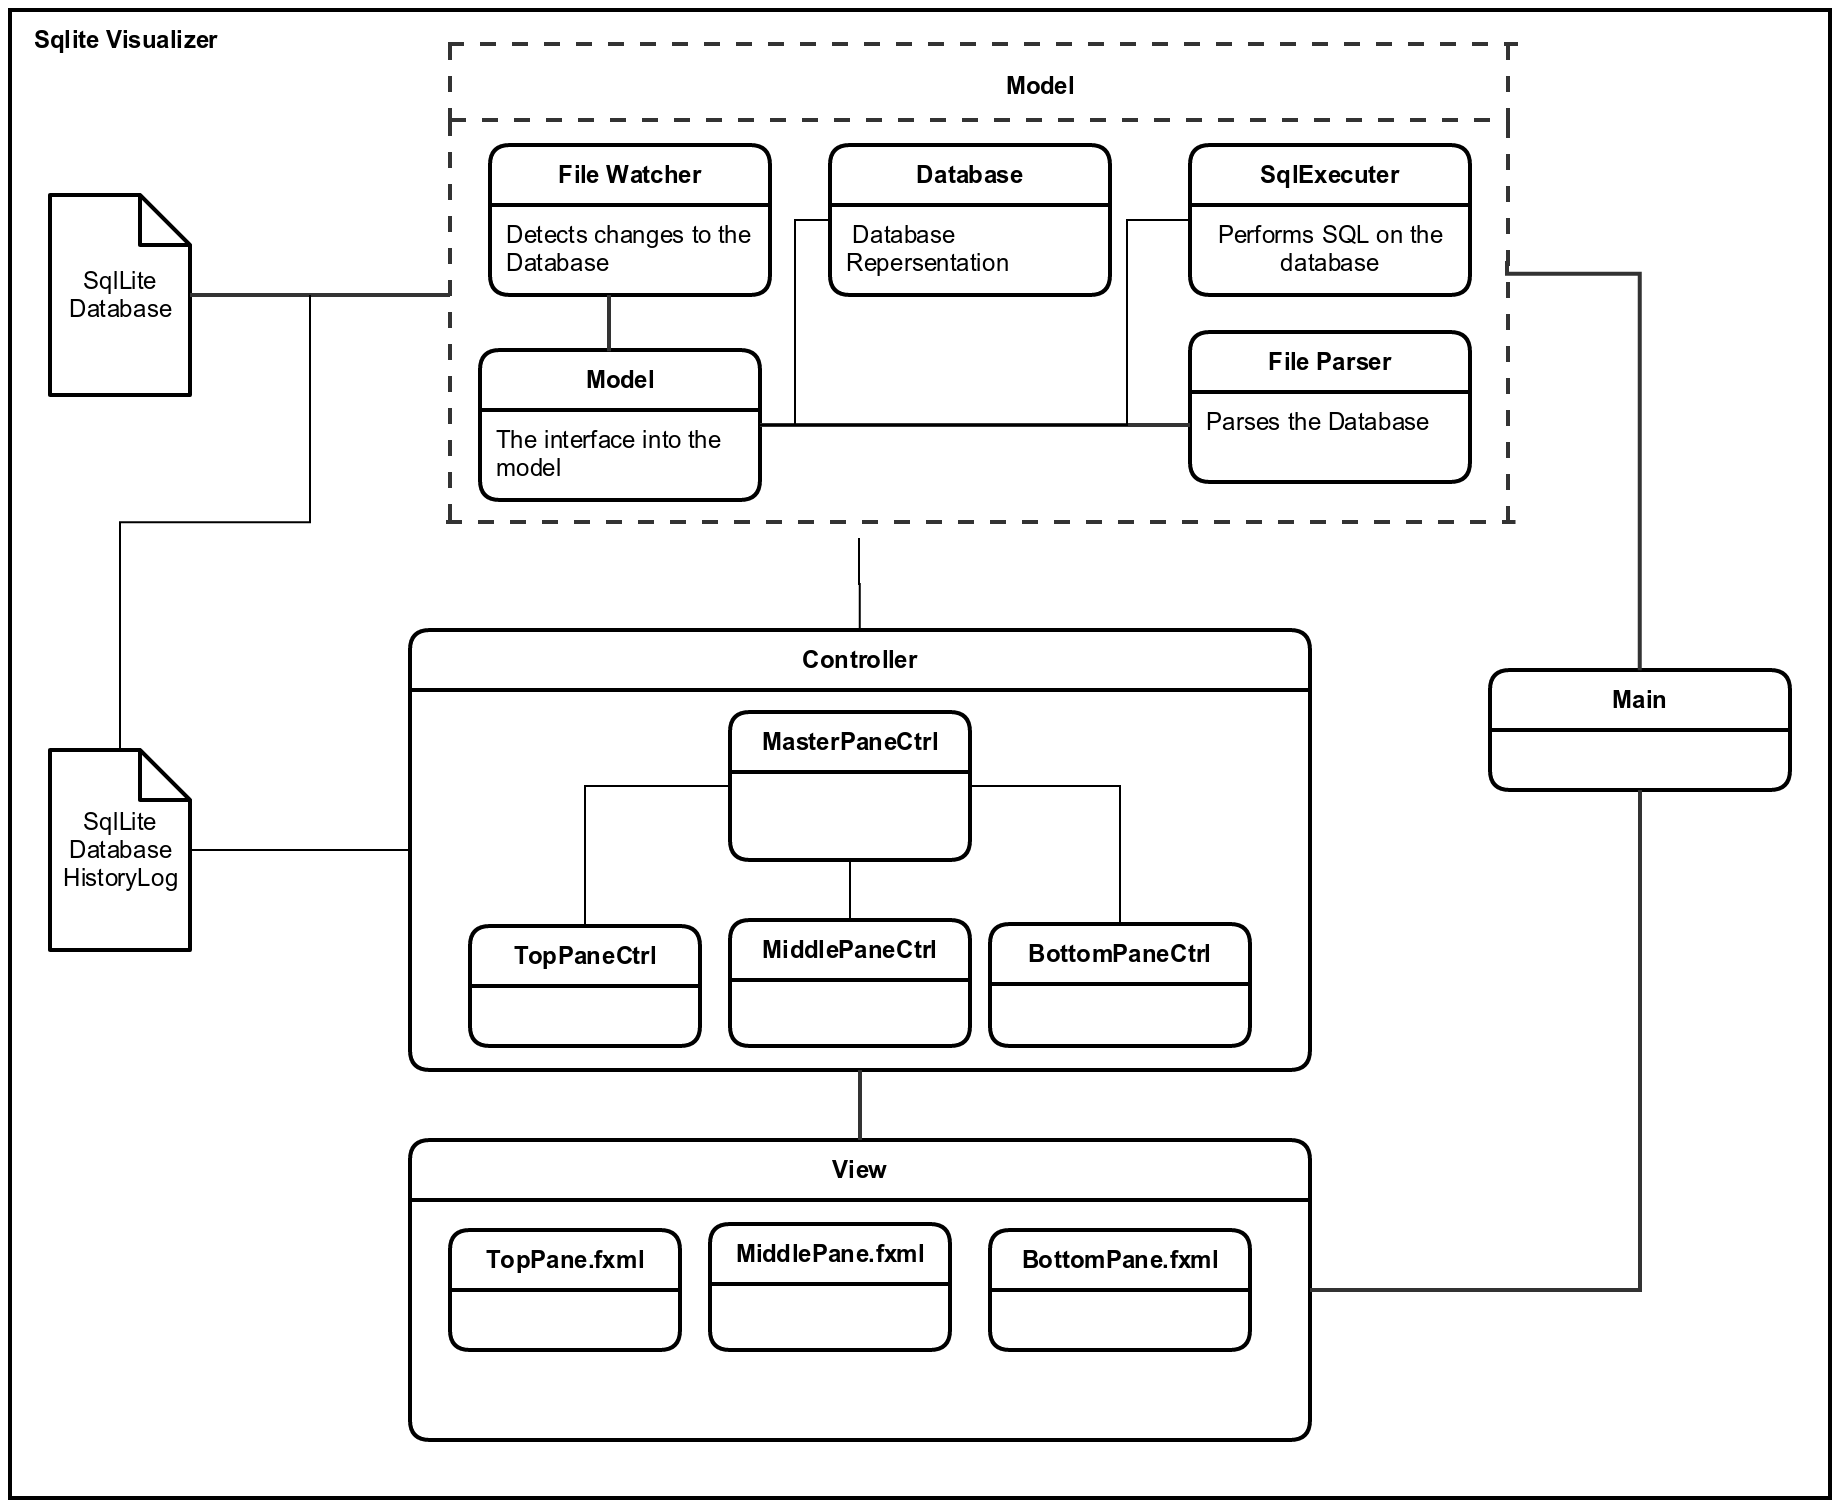
\includegraphics[scale=0.2]{images/system_diagram_old.png}
	\caption{Original system diagram}
	\label{fig:design_old}
\end{figure}

As you can see, the design utilizes the MVC (Model-View-Controller) style architect in order to separate the interface from the data. This means the view will make requests to the controller, who will then in turn contact the model for information, then sending the information to be presented by the view. The idea being that the view could be switched or adjusted at anytime without breaking the application. an example of MVC can be seen below in figure~\ref{fig:mvc}.

\begin{figure}[H]
	\centering
	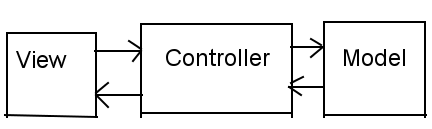
\includegraphics[scale=0.5]{images/mvc.png}
	\caption{MVC architecture}
	\label{fig:mvc}
\end{figure}

The Model was going to run in its own thread so it could control, manage and prepare the data as it came in. This meant the view could request it when it wanted. One other thing to note, is the command logging was going to store them in to an external file, for the view. However, this design proved unusable and thus changed into the following seen in figure~\ref{fig:design_new}. 

\begin{figure}[H]
	\centering
	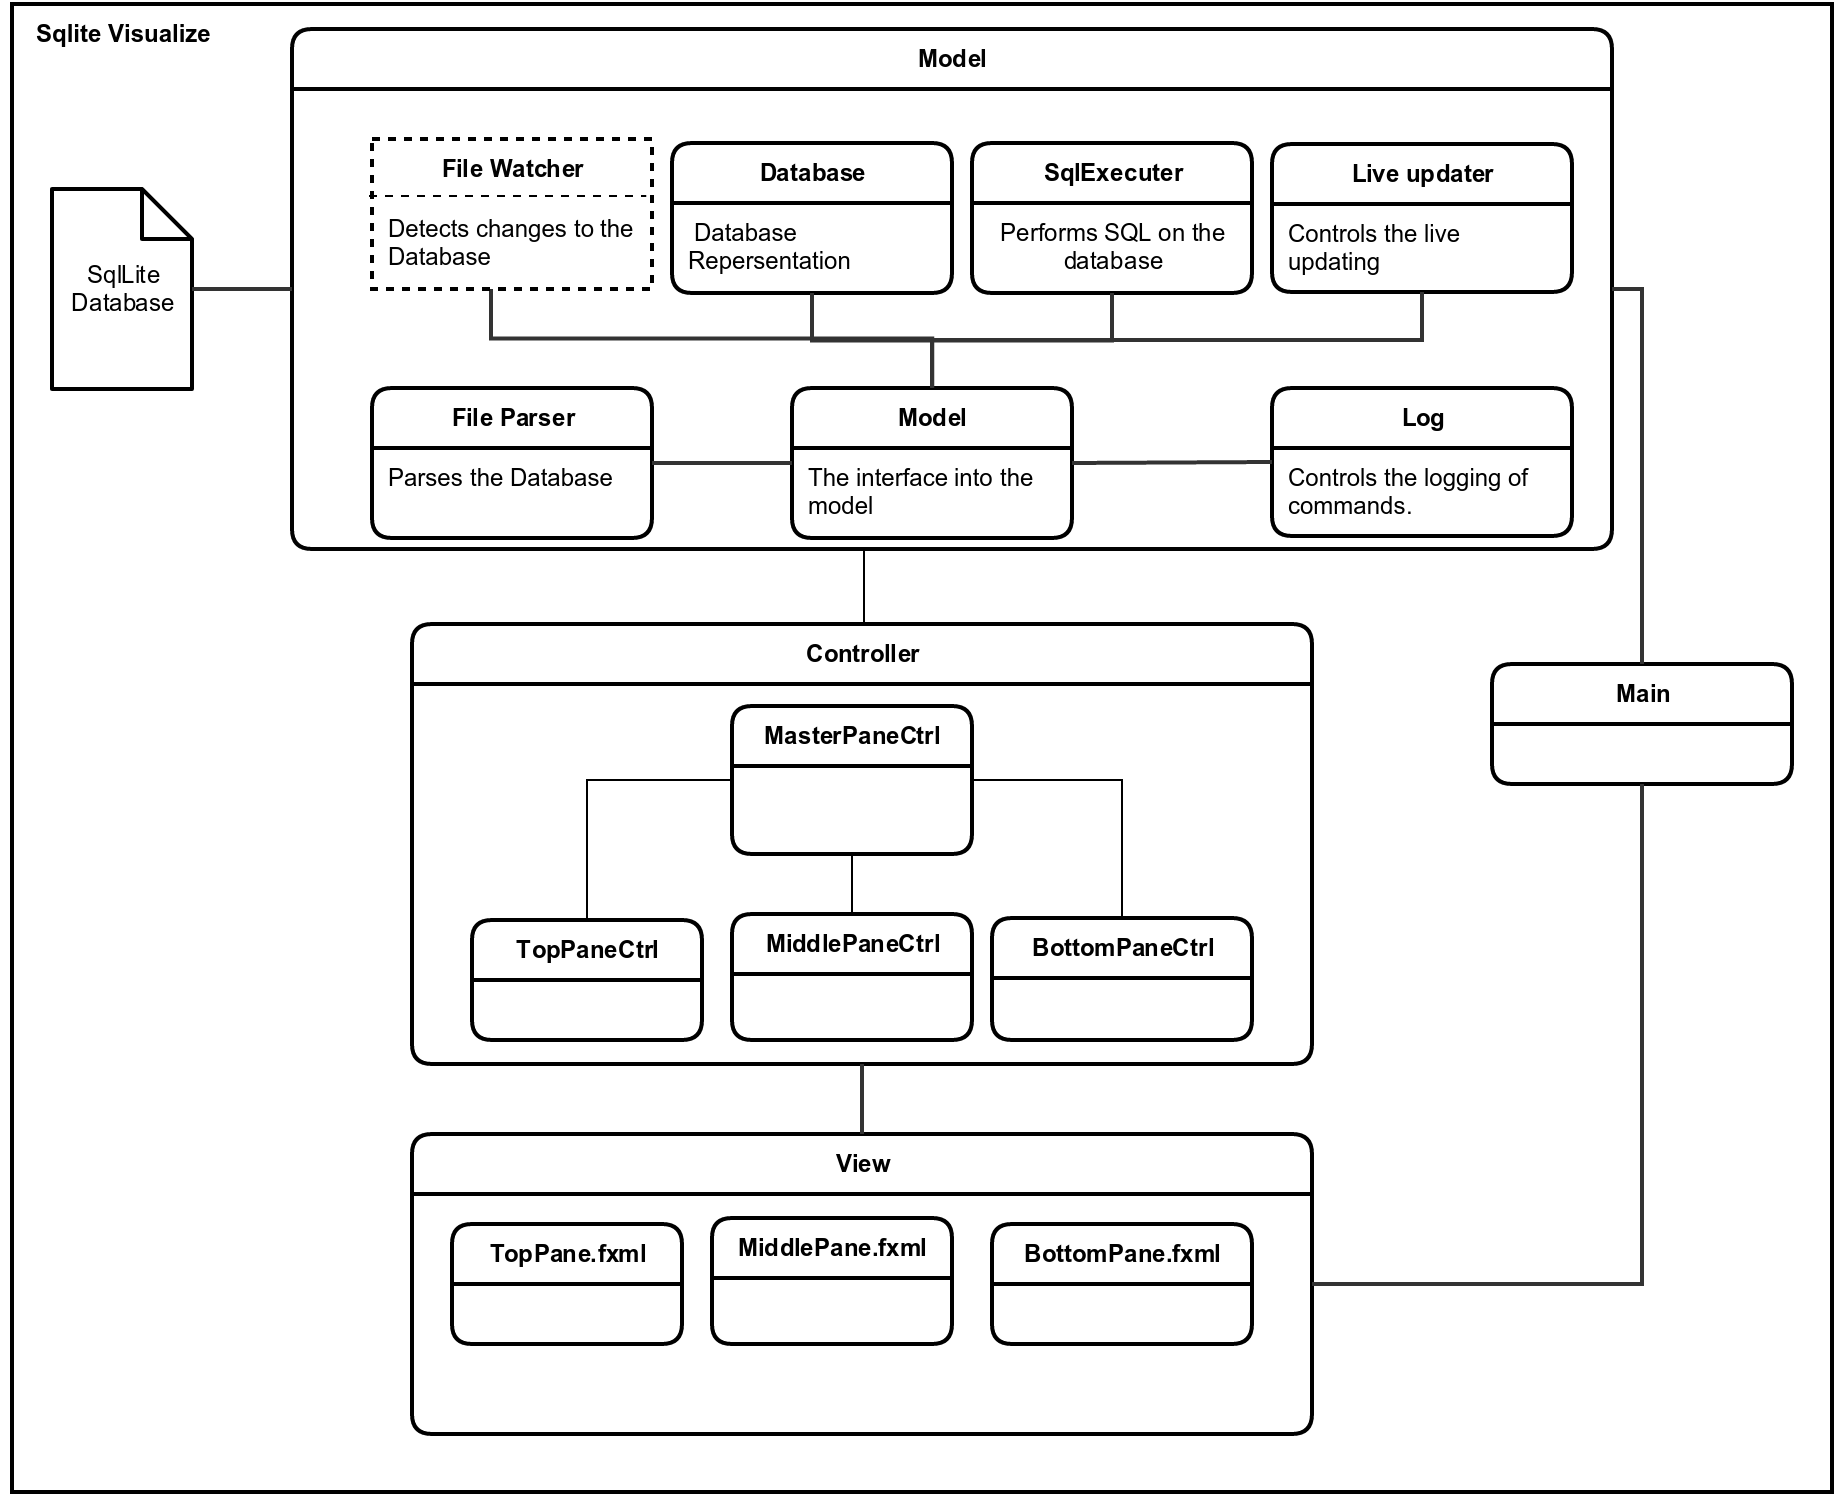
\includegraphics[scale=0.2]{images/system_diagram_new.png}
	\caption{Final system diagram}
	\label{fig:design_new}
\end{figure}

Most of the changes are seen within the Model, with the addition of two new modules. And rather then running the whole thing inside a new thread only the file watcher is. On top of this the command logging is no longer written out to file. The final change is the reduction in the amount of controllers. I will go over each of the modules in the next part.

\subsection{Module Overview}
\label{subsec:module_overview}

\subsubsection{The Main}
\label{subsubsec:main}

The main module represent the staring point of the application, it serves no other purpose other then to correctly initialise the view, model and controllers.

\subsubsection{The View}
\label{subsubsec:the_view}

The view, consists of three parts, the top, middle and right side. Since it follows the MVC style, these only contain the layout of each of the corresponding sections. The middle section however, changes depending on what is being viewed.

\subsubsection{The Controller}
\label{subsubsec:the_controller}

The controller is made up of two parts, the master controller, and the pane controller. The pane controller is changed depending on what is being viewed. Similar to the views middle pane. The master controller coordinates what is being shown. Both of them communicate to the model to collect updates, and interact with the data.

\subsubsection{The Model}
\label{subsubsec:the_model}

The model is the most complicated section and is made up of seven modules. The model itself acts as a repository design with everything connecting and interacting though it.
\\\\
All contact with the model will go though the model interface. This allows the controllers to communicate to the individual modules. In addition to this, it provides a small amount of functionality for setting up and closing. Such as opening the database. Since every module will require something from this action, the model interface will take care of setting up each module. And on exit making sure all threads have been stopped, and any other connections have been closed.
\\\\
The Database, is the in program mapping of the SQLite database system. The database is made up of two parts, the data objects, and the interface into the data object. The data object are the mapping of the SQLite database. Containing the B-Tree system, and the data. The interface provides access to the history, allowing to program move along the database time line. And management of the data objects.
\\\\
The file watcher, runs in its own thread, and utilises the observer pattern. It runs in a continuous loop waiting for a modification to happen on the database. Once a change is detect it sends a signal out over the observers, so the change is recorded. Although, if they did not tune in to the observer, the rest of the program would not receive database updates.
\\\\
The File parser, parses any given valid database file. Converting it into the database object.
\\\\
The log, takes any two database objects and records the changes between them.
\\\\
The live updater, acts like a master controller for the modules, apart from the SQL executor, file watcher and model interface. It controls what happens when a change is detected, and as such is registered to the file watchers observer. When a change is detected, the first thing it does is contact the file parser for the updated database object, send it off to the log, to record changes, and then stores it in the database module. As it controls what happens and when it can also not update, allowing the parsing to pause.
\\\\
The SQL executor, controls the SQL connections, and executes SQL commands onto the database.

\subsection{The User interface}
\label{subsec:high_user_interface}
***************************************************\\
TODO: WHEN FINISHED!\\
****************************************************